%%%%%%%%%%%%%%%%%
% (v1.1.5, 1 December 2018) written by LianTze Lim (liantze@gmail.com). Now compiles with pdfLaTeX, XeLaTeX and LuaLaTeX.
%
%% It may be distributed and
%%or modified under the
%% conditions of the LaTeX Project Public License, either version 1.3
%% of this license or (at your option) any later version.
%% The latest version of this license is in
%%    http://www.latex-project.org/lppl.txt
%% and version 1.3 or later is part of all distributions of LaTeX
%% version 2003/12/01 or later.
%%%%%%%%%%%%%%%%

%% If you need to pass whatever options to xcolor
\PassOptionsToPackage{dvipsnames}{xcolor}

%% If you are using \orcid or academicons
%% icons, make sure you have the academicons
%% option here, and compile with XeLaTeX
%% or LuaLaTeX.
% \documentclass[10pt,a4paper,academicons]{altacv}

%% Use the "normalphoto" option if you want a normal photo instead of cropped to a circle
% \documentclass[10pt,a4paper,normalphoto]{altacv}

\documentclass[10pt,a4paper,ragged2e]{altacv}

%% AltaCV uses the fontawesome and academicon fonts
%% and packages.
%% See http://texdoc.net/pkg/fontawesome and http://texdoc.net/pkg/academicons for full list of symbols. You MUST compile with XeLaTeX or LuaLaTeX if you want to use academicons.

% Change the page layout if you need to
\geometry{left=1.25cm,right=1.25cm,top=1.5cm,bottom=1.5cm,columnsep=1.2cm}

% The paracol package lets you typeset columns of text in parallel
\usepackage{paracol}

% Change the font if you want to, depending on whether
% you're using pdflatex or xelatex/lualatex
\ifxetexorluatex
  % If using xelatex or lualatex:
  \setmainfont{Lato}
\else
  % If using pdflatex:
  \usepackage[utf8]{inputenc}
  \usepackage[T1]{fontenc}
  \usepackage[default]{lato}
\usepackage{biblatex}
\fi

% Change the colours if you want to
\definecolor{Mulberry}{HTML}{72243D}
\definecolor{SlateGrey}{HTML}{2E2E2E}
\definecolor{LightGrey}{HTML}{666666}
\colorlet{heading}{Sepia}
\colorlet{accent}{Mulberry}
\colorlet{emphasis}{SlateGrey}
\colorlet{body}{LightGrey}

% Change the bullets for itemize and rating marker
% for \cvskill if you want to
\renewcommand{\itemmarker}{{\small\textbullet}}
\renewcommand{\ratingmarker}{\faCircle}
\linespread{0.9}
%% sample.bib contains your publications
\addbibresource{sample.bib}

\begin{document}
\name{\LARGE Cheat-Sheet: Virtualisierung}
\tagline{\normalsize Virtualisierung ist eine Hardware-Unterstützung, die den Betrieb virtueller Computer auf einem echten Computer erleichtert oder beschleunigt. Mit der Virtualisierung kann man mehrere Software-Systeme auf einer Hardware laufen lassen. Das können zum Beispiel unterschiedliche Betriebssysteme sein. Virtualisierung macht dann Sinn, wenn ein Hardware-System nicht ausgelastet ist und die Ressourcen parallel für weitere Systeme genutzt werden sollen.}

  %% You MUST add the academicons option to \documentclass, then compile with LuaLaTeX or XeLaTeX, if you want to use \orcid or other academicons commands.
  % \orcid{orcid.org/0000-0000-0000-0000}

\makecvheader

%% Depending on your tastes, you may want to make fonts of itemize environments slightly smaller
% \AtBeginEnvironment{itemize}{\small}

%% Set the left/right column width ratio to 6:4.
\columnratio{0.5}

% Start a 2-column paracol. Both the left and right columns will automatically
% break across pages if things get too long.
\begin{paracol}{2}
\cvsection{\Large Vor- und Nachteile}

\cvevent{Vorteile}{}{}{}
\begin{itemize}
\item Arbeitsspeicher und CPU werden konstanter ausgelastet, nicht nur bei Server-Spitzen.
\item Eine VM ist schnell wiederhergestellt.\newline Auf Host-Ebene sind alle virtuellen Maschinen \newline gemeinsam sicherbar.
\item Mit wenig Aufwand, kann ein weiterer Host \newline / Server / virtueller Desktop aufgesetzt und die VMs repliziert werden.  
\item Gesamtes System, auch virtuelle Server mit einem Programm verwaltbar.

\end{itemize}

\vspace{3mm}

\cvevent{Nachteile}{}{}{}
\begin{itemize}
\item Wenn die Bandbreite des eigenen Netzwerkes nicht ausreichend, mögliche "Verstopfung" der Leitung.
\item Wenn ein Server nicht genug Leistung hat, \newline muss nachgerüstet werden. (Kosten)
\item Es werden trotz Virtualisierung Desktop-Rechner benötigt. Ob zur Verwaltung der virtuellen Maschinen, oder für Arbeitsplätze.

\end{itemize}

\cvsection{\Large Definitionen}

\cvevent{Hypervisor / VMM (VM-Monitor)}{}{}{}
\begin{itemize}
\item Weist den verschiedenen virtuellen Instanzen die Hardware Ressourcen zu und verwaltet Isolation der virtuellen Systeme untereinander.
\end{itemize}

\vspace{3mm}

\cvevent{Gast}{}{}{}
\begin{itemize}
    \item Eigene Instanz innerhalb des Hosts 
\end{itemize}

\vspace{3mm}

\cvevent{Wirt (Host)}{}{}{}
\begin{itemize}
    \item Bietet dem VMM die nötigen Resourcen zum verwalten.
\end{itemize}

\vspace{3mm}

\cvevent{Virtuelle Maschine (VM)}{}{}{}
\begin{itemize}
    \item Emulation eines Betriebssystems
\end{itemize}

\vspace{3mm}

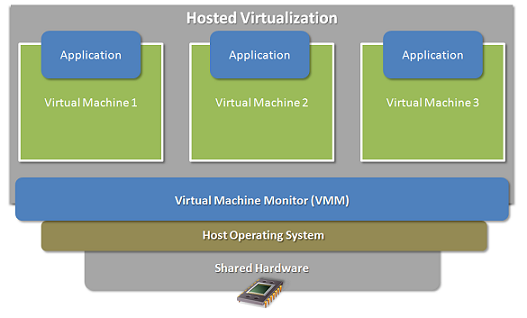
\includegraphics[width=0.48\textwidth]{Hosted.PNG}

\newpage
\begin{thebibliography}{9}

\bibitem{typeReference} 
Arten der Virtualisierung,
\\\texttt{https://www.cloudcomputing-insider.de\newline/was-ist-virtualisierung-a-756279/}

\end{thebibliography}

\switchcolumn

\cvsection{\Large Arten}

\cvachievement{\faDesktop}{Desktopvirtualisierung}{
    \begin{itemize}
        \item Abbild des Arbeitsplatzes zentral im Rechenzentrum Verfügbar.
        \item Anwender verbindet sich mit dem Image im Rechenzentrum
        \item Je System und Strategie ist ein dediziertes Image möglich oder alle/eine Gruppe von Mitarbeitern, nutzt ein gemeinsames Image.
    \end{itemize}
}

\cvachievement{\faServer}{Server Virtualisierung}{
    \begin{itemize}
        \item Gemeinsame Nutzung der Host-Ressourcen
        \item Ressourcenverwaltung durch Software möglich
        \item Kann auf andere Host-Systeme verschoben werden
    \end{itemize}
}
\cvachievement{\faWindows}{Betriebssysteme Virtualisierung}{
    Andere Betriebssysteme sind auf dem Host-Betriebssystem parallel ausführbar \newline
}


\cvachievement{\faDatabase}{Speichervirtualisierung }{
    \begin{itemize}
        \item Virtuelle Bereitstellung von Speicherplatz
        \item Erstreckt sich über mehrere physische Storage-Geräte
        \item Spricht nur den virtualisierten Speicher an
        \item Virtualisierungssoftware sorgt für die physikalische Speicherung der Daten.
    \end{itemize}
}
\cvachievement{\faWifi}{Netzwerkvirtualisierung}{
    \begin{itemize}
        \item Trennt die Netzwerkfunktionen von den physischen Systemen
        \item Reduziert Anzahl an physischen Systemen, da auf gemeinsamen Host-Systemen virtuell bereitgestellt. 
        \item (SDN) Hoher Grad der Virtualisierung, trennt die Netzwerksoftware von Netzwerkhardware.
    \end{itemize}
}

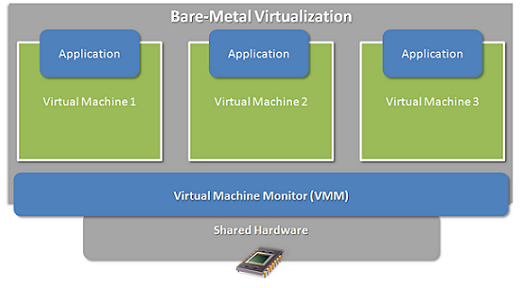
\includegraphics[width=0.48\textwidth]{Bare.PNG}
\footnote{Der Bare-Metal-Typ kann ohne weitere Software mit der Hardware kommunizieren und setzt nicht wie der Host-Typ auf einem vollwertigen Betriebssystem auf.}

\end{paracol}

\end{document}
